%%%%    Davor Penzar --- Diplomski rad.

% Klasa dokumenta: beamer.
\documentclass[croatian, 12pt, usepdftitle = false, xcolor = {{usenames, dvipsnames, svgnames, x11names}}, hyperref = {unicode}]{beamer}
    \mode<presentation>

% Neke opcije za "kvalitetniji" (barem u smislu eksportiranja teksta) PDF dokument.
\pdfinterwordspaceon
\input{glyphtounicode}
\pdfgentounicode=1

% Stil za diplomski rad.
\usepackage{packages/obrana}
    \pgfplotsset{compat = 1.15}
    \hypersetup{
        hidelinks,
        pdfstartview = ,
        pdftitle = {Metode strojnog u\v{c}enja u predvi{\dj}anju najni\v{z}e svojstvene vrijednosti Laplaceovog operatora},
        pdfauthor = {Davor Penzar},
        pdfsubject = {Diplomski rad},
        pdfkeywords = {strojno u\v{c}enje, duboko strojno u\v{c}enje, linearna regresija, neurosnke mre\v{z}e, konvolucijske neuronske mre\v{z}e, Dirichletov Laplaceov operator, svojstvena vrijednost Dirichletovog Laplaceovog operatora}
    }

% Paket s prosirenom podrskom "masnih" znakova.
%\usepackage{bbm}

% Paket sa simbolima kao tekstualnim znakovima.
\usepackage{pifont}

% Paket za prikaz rubova dijelova stranica (zaglavlje, glavni dio, podnozje).
%\usepackage{showframe}

% Paket za generiranje "lorem ipsum" teksta.
\usepackage{lipsum}

% Dopustanje prekida stranica u matematickim okruzenjima.
\allowdisplaybreaks

% Podatci o diplomskom radu.
\title[Obrana diplomskog rada]{Metode strojnog u\v{c}enja u predvi{\dj}anju najni\v{z}e svojstvene vrijednosti Laplaceovog operatora}
\subtitle{Diplomski rad}
\author[Davor Penzar]{Davor Penzar \\ {\small Voditelj rada: prof.\ dr.\ sc.\ Luka Grubi\v{s}i\'{c}}}
\institute[]{\href{https://www.math.pmf.unizg.hr/hr}{Matemati\v{c}ki odsjek} \\ \href{https://www.pmf.unizg.hr/}{Prirodoslovno-matemati\v{c}ki fakultet} \\ \href{http://www.unizg.hr/}{Sveu\v{c}ili\v{s}te u Zagrebu}}
\date[Zagreb, {$ \mathsf{\numprint{2020}} $.}]{Zagreb, \DTMdate{2020-02-28}}
%\logo{
\includegraphics[width = 15mm]{PMF-logo.pdf}}

% Literatura.
\addbibresource{bibliography/bibliography.bib}

% Definicija naredbe za oznaku kompleksno konjugiranog broja.
\newcommand*{\conjugate}[1]{\overline{#1}}

% Definicija naredbe za oznaku restrikcije funkcije.
\newcommand*{\restrictlparen}{.}
\newcommand*{\restrictmparen}{|}
\newcommand*{\restrictrparen}{.}
\newcommand*{\restrict}[2]{\left\restrictlparen {#1} \restrictmparen_{{#2}} \right\restrictrparen}

% Definicija naredbe za oznaku faktorijela.
\newcommand*{\factorial}{!}

% Definicija naredbe za oznaku karakteristicne funkcije.
\newcommand*{\characteristicfont}{\mathit}
\newcommand*{\characteristicsym}{\chi}
\DeclareMathOperator{\characteristicop}{\characteristicfont{\characteristicsym}}
\newcommand*{\characteristic}[1]{\characteristicop_{{#1}}}

% Definicija naredbe za oznaku Kroneckerove delta-funkcije.
\newcommand*{\Kroneckerdsym}{\delta}
\newcommand*{\Kroneckerd}[2]{\Kroneckerdsym_{{#1} , {#2}}}

% Definicije naredbi za oznake najveceg cijelog, najmanjeg cijelog i decimalnog dijela.
\newcommand*{\floorlparen}{\lfloor}
\newcommand*{\floorrparen}{\rfloor}
\newcommand*{\ceillparen}{\lceil}
\newcommand*{\ceilrparen}{\rceil}
\newcommand*{\fracpartlparen}{\{}
\newcommand*{\fracpartrparen}{\}}
\newcommand*{\floor}[1]{\left\floorlparen {#1} \right\floorrparen}
\newcommand*{\ceil}[1]{\left\ceillparen {#1} \right\ceilrparen}
\newcommand*{\fracpart}[1]{\left\fracpartlparen {#1} \right\fracpartrparen}

% Definicije naredbi za notaciju redova veliko O i malo o.
\newcommand*{\onotefont}{\mathcal}
\newcommand*{\littleosym}{o}
\newcommand*{\bigOsym}{O}
\DeclareMathOperator{\bigO}{\onotefont{\bigOsym}}
\DeclareMathOperator{\littleo}{\onotefont{\littleosym}}

% Definicije naredbi za interior, zatvorenje i rub skupa.
\newcommand*{\interiorfont}{\mathrm}
\newcommand*{\interiorsym}{Int}
\DeclareMathOperator{\interior}{\interiorfont{\interiorsym}}
\DeclareMathOperator{\boundary}{\partial}
\newcommand*{\closure}[1]{\overline{#1}}

% Definicija naredbe za oznaku metrike.
\newcommand*{\normlparen}{\lVert}
\newcommand*{\normrparen}{\rVert}
\newcommand*{\norm}[1]{\left\normlparen {#1} \right\normrparen}

% Definicija naredbe za oznaku udaljenosti.
\newcommand*{\distancefont}{\mathit}
\newcommand*{\distancesym}{d}
\DeclareMathOperator{\distanceop}{\distancefont{\distancesym}}
\newcommand*{\distance}[2]{\distanceop \left( {#1} , {#2} \right)}
\newcommand*{\Distance}[3]{\distanceop^{{#3}} \left( {#1} , {#2} \right)}

% Definicija naredbe za onaku otvorene kugle.
\newcommand*{\openballfont}{\mathit}
\newcommand*{\openballsym}{B}
\DeclareMathOperator{\openballop}{\openballfont{\openballsym}}
\newcommand*{\openball}[2]{\openballop_{#2} \left( {#1} \right)}

% Definicija naredbe za oznaku dijametra skupa.
\newcommand*{\diameterfont}{\mathit}
\newcommand*{\diametersym}{d}
\DeclareMathOperator{\diameter}{\diameterfont{\diametersym}}

% Definicija naredbe za oznaku funkcije dubine poligona.
\newcommand*{\deepnessfont}{\mathit}
\newcommand*{\deepnesssym}{D}
\DeclareMathOperator{\deepness}{\deepnessfont{\deepnesssym}}

% Definicija naredbe za oznake pravca kroz dvije tocke i duzine izmedu dvije tocke.
\newcommand*{\lengthlparen}{\lvert}
\newcommand*{\lengthrparen}{\rvert}
\newcommand*{\straightline}[2]{{{#1} {#2}}}
\newcommand*{\linesegment}[2]{\overline{{#1} {#2}}}
\newcommand*{\linesegmentlength}[2]{\left\lengthlparen \linesegment{{#1}}{{#2}} \right\lengthrparen}

% Definicija naredbe za oznaku trokuta zadanog trima tockama.
\newcommand*{\deftrianglefont}{\mathrm}
\newcommand*{\deftrianglesym}{\bigtriangleup}
\newcommand*{\deftriangleop}{\deftrianglefont{\deftrianglesym}}
\newcommand*{\deftriangle}[3]{\deftriangleop {{#1} {#2} {#3}}}

% Definicije naredbi za lijevi i desni limes.
\newcommand*{\llimitexp}{{-}}
\newcommand*{\rlimitexp}{{+}}
\newcommand*{\llimitpt}[1]{{#1}^{\llimitexp}}
\newcommand*{\rlimitpt}[1]{{#1}^{\rlimitexp}}

% Definicije naredbi za diferencijale.
\newcommand*{\difffont}{\mathrm}
\newcommand*{\diffsym}{d}
\newcommand*{\partdiffsym}{\partial}
\DeclareMathOperator{\derivativeop}{\difffont{\diffsym}}
\DeclareMathOperator{\partialderivativeop}{\partdiffsym}
\newcommand*{\diff}{\mathop{}\!\difffont{\diffsym}}
\newcommand*{\Diff}[1]{\mathop{}\!\difffont{\diffsym}^{{#1}}}
\newcommand*{\derivative}[1]{\frac{\difffont{\diffsym}}{\derivativeop {#1}}}
\newcommand*{\Derivative}[2]{\frac{\difffont{\diffsym}^{{#2}}}{\derivativeop {#1}^{{#2}}}}
\newcommand*{\DerivativeSub}[3]{\frac{\difffont{\diffsym}^{{#3}}}{\derivativeop {#1}_{{#2}}^{{#3}}}}
\newcommand*{\partialderivative}[1]{\frac{\partdiffsym}{\partialderivativeop {#1}}}
\newcommand*{\PartialDerivative}[2]{\frac{\partdiffsym^{{#2}}}{\partialderivativeop {#1}^{{#2}}}}
\newcommand*{\PartialDerivativeSub}[3]{\frac{\partdiffsym^{{#3}}}{\partialderivativeop {#1}_{{#2}}^{{#3}}}}

% Definicije naredbi za gradijent i divergenciju.
\newcommand*{\gradientfont}{\mathrm}
\newcommand*{\divergencefont}{\mathrm}
\newcommand*{\gradientsym}{grad}
\newcommand*{\divergencesym}{div}
\DeclareMathOperator{\gradient}{\gradientfont{\gradientsym}}
\DeclareMathOperator{\divergence}{\divergencefont{\divergencesym}}

% Definicija naredbe za oznaku Laplaceovog operatora (Laplaciana).
\DeclareMathOperator{\Laplacian}{\Delta}

% Definicije naredbi za klase neprekidnih funkcija.
\newcommand*{\continuousfont}{\mathit}
\newcommand*{\continuoussym}{C}
\DeclareMathOperator{\continuousop}{\continuousfont{\continuoussym}}
\newcommand*{\continuous}[2]{\continuousop^{{#2}} \left( {#1} \right)}
\newcommand*{\Continuous}[3]{\continuous{{#1} , {#2}}{#3}}

% Definicije naredbi za oznake vektora, linearnih operatora i matrica.
\newcommand*{\vectorspacefont}{\mathit}
\newcommand*{\vectorfont}{\mathbf}
\newcommand*{\linearspacefont}{\mathit}
\newcommand*{\linearfont}{\mathit}
\newcommand*{\matrixalgebrafont}{\mathrm}
\newcommand*{\matrixfont}{\mathit}
\newcommand*{\vectorspacesym}{V}
\newcommand*{\linearspacesym}{L}
\newcommand*{\matrixalgebrasym}{M}
\DeclareMathOperator{\vectorspaceop}{\vectorspacefont{\vectorspacesym}}
\newcommand*{\vectorspace}{\VectorSpace{\vectorspaceop}}
\newcommand*{\VectorSpace}[1]{\VectorSpacen{\vectorspaceop}^{{#1}}}
\DeclareMathOperator{\linearspaceop}{\linearspacefont{\linearspacesym}}
\newcommand*{\linearspace}[1]{\linearspaceop \left( {#1} \right)}
\newcommand*{\LinearSpace}[2]{\linearspace{{#1} , {#2}}}
\DeclareMathOperator{\matrixalgebraop}{\matrixalgebrafont{\matrixalgebrasym}}
\newcommand*{\matrixalgebra}[1]{\matrixalgebraop_{{#1}}}
\newcommand*{\matrixalgebramn}[2]{\matrixalgebra{{#1} , {#2}}}
\newcommand*{\MatrixAlgebra}[2]{\matrixalgebra{{#2}} \left( {#1} \right)}
\newcommand*{\MatrixAlgebramn}[3]{\matrixalgebramn{{#2}}{{#3}} \left( {#1} \right)}
\newcommand*{\aslinear}[1]{\linearfont{{#1}}}
\newcommand*{\asvector}[1]{\vectorfont{{#1}}}
\newcommand*{\asmatrix}[1]{\matrixfont{{#1}}}

% Definicija naredbe za oznaku vektora izmedu dvije tocke.
\newcommand*{\vectorline}[2]{\overrightarrow{{#1} {#2}}}

% Definicija naredbi za oznake transponenta i hermitske adjunkte matrice.
\newcommand*{\transponent}{{\mathchar"AFC}}
\newcommand*{\Hermiteconjugate}{{*}}

% Definicija naredbe za skalarni produkt.
\newcommand*{\dotproductlparen}{\langle}
\newcommand*{\dotproductrparen}{\rangle}
\newcommand*{\dotproductdelim}{,}
\newcommand*{\dotproduct}[2]{\left\dotproductlparen {#1} \dotproductdelim {#2} \right\dotproductrparen}

% Definicija naredbe za oznaku spektra.
\DeclareMathOperator{\spectrum}{\sigma}

% Definicija okruzenja za sustav jednadzbi.
\newenvironment{eqsystem}{%
    \left\{%
    \begin{array}{r @{\;} l l}%
    \displaystyle%
}
{%
    \end{array}%
    \right.%
}

% Definiranje vlastitog stila programskih kodova.
\lstdefinestyle{program}
{
    breaklines = true,
    breakatwhitespace = true,
    numbers = left,
    stepnumber = 1,
    numberstyle = {\footnotesize \ttfamily \bfseries},
    tabsize = 4,
    frame = none,
    basicstyle = {\ttfamily},
    stringstyle = {\color{red}},
    keywordstyle = {\bfseries \color{blue}},
    commentstyle = {\itshape \color{gray}},
    showstringspaces = true
}

% Definicija naredbe za referenciranje i citiranje kao "v. [izvor]".
\newcommand*{\seetxt}{v.}
\newcommand*{\Seetxt}{V.}
\newcommand*{\seeref}[1]{\seetxt~\ref{#1}}
\newcommand*{\Seeref}[1]{\Seetxt~\ref{#1}}
\newcommand*{\seecite}[1]{\seetxt~\cite{#1}}
\newcommand*{\Seecite}[1]{\Seetxt~\cite{#1}}

% Definicija naredbe za naglasavanje definiranog pojma u definiciji.
\newcommand*{\defined}[1]{\emph{#1}}

\begin{document}
    \frame{\titlepage}

    \frame{\tableofcontents}

    \section{Svojstvene vrijednosti i svojstvene funkcije Laplaceovog operatora}

    \begin{frame}{Svojstvene vrijednosti i svojstvene funkcije Laplaceovog operatora}
        \begin{definition}
            $ u $ je \defined{svojstvena funkcija}, a $ \lambda $ \defined{svojstvena vrijednost} Laplaceovog operatora na nepraznom, otvorenom i ograničenom skupu $ \Omega $ t.\ d.\ je $ \boundary \Omega $ po djelovima gladak ako je
            \begin{itemize}
                \item $ u \colon \closure{\Omega} \to \reals $ neprekidna na $ \closure{\Omega} $, dvaput diferencijabilna na $ \Omega $
                \item $ \lambda \in \reals \setminus \left\{ \numprint{0} \right\} $
            \end{itemize}
            i vrijedi
            \begin{equation} \label{eq:Dirichlet_Laplacian_problem}
                \begin{eqsystem}
                    {- {\Laplacian u}} & = \lambda u \text{,} & \text{na} \ \Omega \text{,} \\
                    u & = \numprint{0} \text{,} & \text{na} \ \boundary \Omega
                \end{eqsystem}
            \end{equation}

            \par

            \defined{Spektar} skupa $ \Omega $ je
            \begin{equation*}
                \spectrum \left( \Omega \right) \coloneqq \left( \lambda_{i} \right)_{i \in \positives{\naturals}} , \quad \numprint{0} < \lambda_{\numprint{1}} \leq \lambda_{\numprint{2}} \leq \dotsb \leq \lambda_{k} \leq \dotsb \uparrow {+ \infty}
            \end{equation*}

            \par
        \end{definition}
    \end{frame}

    \begin{frame}{Normalizacija skupa}
        \begin{theorem}
            Neka su $ \Omega_{\numprint{1}} , \Omega_{\numprint{2}} \subseteq \reals^{n} $ proizvoljni t.\ d.\ zadovoljavaju uvjete iz definicije svojstvenih vrijednosti i svojstvenih funkcija Laplaceovog operatora. Tada vrijedi
            \begin{equation*}
                \Omega_{\numprint{1}} \sim \Omega_{\numprint{2}} \implies \diameter^{\numprint{2}} \left( \Omega_{\numprint{1}} \right) \spectrum \left( \Omega_{\numprint{1}} \right) = \diameter^{\numprint{2}} \left( \Omega_{\numprint{2}} \right) \spectrum \left( \Omega_{\numprint{2}} \right) \text{.}
            \end{equation*}
        \end{theorem}
    \end{frame}

    \begin{frame}{Monotonost svojstvenih vrijednosti Laplaceovog operatora}
        \begin{proposition}
            Neka su $ \Omega_{\numprint{1}} , \Omega_{\numprint{2}} \subseteq \reals^{n} $ proizvoljni t.\ d.\ zadovoljavaju uvjete iz definicije svojstvenih vrijednosti i svojstvenih funkcija Laplaceovog operatora. Tada vrijedi
            \begin{equation*}
                \Omega_{\numprint{1}} \subseteq \Omega_{\numprint{2}} \implies \forall k \in \positives{\naturals} \left( \lambda_{k} \left( \Omega_{\numprint{1}} \right) \geq \lambda_{k} \left( \Omega_{\numprint{2}} \right) \right) \text{.}
            \end{equation*}
            To jest, za svaki $ k \in \positives{\naturals} $ parcijalno preslikavanje $ \lambda_{k} \colon \powerset \left( \reals^{n} \right) \partto \intervaloo{\numprint{0}}{{+ \infty}} $ je padajuće s obzirom na inkluziju.
        \end{proposition}
    \end{frame}

    \begin{frame}{Neprekidnost svojstvenih vrijednosti Laplaceovog operatora}
        \only<1>{%
            \begin{theorem}
                Za svaki $ k \in \positives{\naturals} $ parcijalno preslikavanje $ \lambda_{k} \colon \powerset \left( \reals^{n} \right) \partto \intervaloo{\numprint{0}}{{+ \infty}} $ je neprekidno.~\cite[418--424]{bib:Courant53}
            \end{theorem}%
        }%
        \only<2->{%
            \framesubtitle{Značenje male razlike domena u kontekstu zadaće~\eqref{eq:Dirichlet_Laplacian_problem}}

            \centering
            \begin{columns}
                \begin{column}{0.333333333333333\textwidth}
                    \centering
                    \begin{tikzpicture}[scale = 1.5]
                        \filldraw[fill = black, fill opacity = 0.15, draw = black, thick] (0, 0) circle (1);
                    \end{tikzpicture}
                    \\
                    Krug
                \end{column}
                \begin{column}{0.333333333333333\textwidth}
                    \centering
                    \begin{tikzpicture}[scale = 1.5]
                        \scope
                            \clip (-1.025, -1.025) rectangle (1.025, 1.025) (0, 0) circle (0.1);
                            \fill[black, opacity = 0.15] (0, 0) circle (1);
                        \endscope
                        \draw[black, thick] (0, 0) circle (0.1);
                        \draw[black, thick] (0, 0) circle (1);
                    \end{tikzpicture}
                    \\
                    Kružni vijenac
                \end{column}
                \begin{column}{0.333333333333333\textwidth}
                    \centering
                    \begin{tikzpicture}[scale = 1.5]
                        \filldraw[fill = black, fill opacity = 0.15, draw = black, thick] (0, 0) ellipse (1.1 and 0.9);
                    \end{tikzpicture}
                    \\
                    Prava elipsa
                \end{column}
            \end{columns}%
        }%
    \end{frame}

    \section{Poligoni}

    \begin{frame}{Poligoni}
        \begin{definition}
            $ P \subseteq \reals^{\numprint{2}} $ je \defined{poligon} ako
            \begin{itemize}
                \item $ \interior P \neq \emptyset $
                \item $ P $ je ograničen
                \item $ \boundary P $ je jednostavna zatvorena krivulja
                \item postoje $ k \in \naturals $ i točke $ V_{\numprint{1}} , V_{\numprint{2}} , \dotsc , V_{k} \in \reals^{\numprint{2}} $ t.\ d.
                    \begin{equation*}
                        \boundary P = \linesegment{V_{\numprint{1}}}{V_{\numprint{2}}} \cup \linesegment{V_{\numprint{2}}}{V_{\numprint{3}}} \cup \dotsb \cup \linesegment{V_{k - \numprint{1}}}{V_{k}} \cup \linesegment{V_{k}}{V_{\numprint{1}}} \text{,}
                    \end{equation*}
                    pri čemu dužine u gornjoj uniji u parovima nemaju zajedničkih točaka osim eventualno krajnjih---$ P $ je \defined{$ k $-gon}
            \end{itemize}
            $ P $ je \defined{pravi $ k $-gon} ako je $ k \in \naturals $ najmanji koji zadovoljava prethodne uvjete
        \end{definition}
    \end{frame}

    \begin{frame}{Karakterizacija poligona pravim vrhovima}
        \only<1>{%
            \begin{theorem}
                Za svaki poligon $ P \subseteq \reals^{\numprint{2}} $
                \begin{enumerate}
                    \item postoje jedinstveni $ k \in \naturals $, $ k \geq \numprint{3} $, i u parovima različite točke $ V_{\numprint{1}} , V_{\numprint{2}} , \dotsc , V_{k} \in \reals^{\numprint{2}} $ t.\ d.\ je $ P $ pravi $ k $-gon s vrhovima $ V_{\numprint{1}} , V_{\numprint{2}} , \dotsc , V_{k} $,
                    \item uređena $ k $-torka $ \left( V_{i_{\numprint{1}}} , V_{i_{\numprint{2}}} , \dotsc , V_{i_{k}} \in \reals^{\numprint{2}} \right) \in \reals^{\numprint{2} \times k} $ vrhova iz prethodne točke tako da se svaki pojavljuje točno jednom i da su oni poredani u pozitivnom smjeru jedinstvena je do na izbor vrha $ V_{i_{\numprint{1}}} $.
                \end{enumerate}
            \end{theorem}%
        }%
        \only<2->{%
            \framesubtitle{Problemi}

            \centering
            \begin{columns}
                \begin{column}{0.333333333333333\textwidth}
                    \centering
                    \begin{tikzpicture}
                        % Koordinatna mreza.
                        \draw[black, opacity = 0.3, very thin, step = 0.25] (-1.625, -1.625) grid (1.625, 1.625);
                        \draw[black, opacity = 0.3, very thin, step = 0.5] (-1.625, -1.625) grid (1.625, 1.625);
                        \draw[black, opacity = 0.3, thin, step = 1] (-1.625, -1.625) grid (1.625, 1.625);

                        % Koordinatne osi.
                        \draw[blue, thin, ->] (-1.625, 0) -- (1.625, 0) node[black, below left] {$ x $};
                        \draw[red, thin, ->] (0, -1.625) -- (0, 1.625) node[black, below left] {$ y $};

                        % Poligon.
                        \filldraw[fill = black, fill opacity = 0.15, draw = black, thick] (1, -1) -- (1, 1) -- (-1, 1) -- (-0.75, 0) -- (0, 0) -- (-1, -1) -- cycle;

                        % Vrhovi poligona.
                        \fill[black] (-1, -1) circle (0.05) node[below left] {$ V_{\numprint{1}} $};
                        \fill[black] (1, -1) circle (0.05) node[below right] {$ V_{\numprint{2}} $};
                        \fill[black] (1, 1) circle (0.05) node[above right] {$ V_{\numprint{3}} $};
                        \fill[black] (-1, 1) circle (0.05) node[above left] {$ V_{\numprint{4}} $};
                        \fill[black] (-0.75, 0) circle (0.05) node[below left] {$ V_{\numprint{5}} $};
                        \fill[black] (0, 0) circle (0.05) node[below right] {$ V_{\numprint{6}} $};
                    \end{tikzpicture}
                    \\
                    Originalni poligon
                \end{column}
                \begin{column}{0.333333333333333\textwidth}
                    \centering
                    \begin{tikzpicture}
                        % Koordinatna mreza.
                        \draw[black, opacity = 0.3, very thin, step = 0.25] (-1.625, -1.625) grid (1.625, 1.625);
                        \draw[black, opacity = 0.3, very thin, step = 0.5] (-1.625, -1.625) grid (1.625, 1.625);
                        \draw[black, opacity = 0.3, thin, step = 1] (-1.625, -1.625) grid (1.625, 1.625);

                        % Koordinatne osi.
                        \draw[blue, thin, ->] (-1.625, 0) -- (1.625, 0) node[black, below left] {$ x $};
                        \draw[red, thin, ->] (0, -1.625) -- (0, 1.625) node[black, below left] {$ y $};

                        % Poligon.
                        \filldraw[fill = black, fill opacity = 0.15, draw = black, thick] (1, -1) -- (0, 0) -- (0.75, 0) -- (1, 1) -- (-1, 1) -- (-1, -1) -- cycle;

                        % Vrhovi poligona.
                        \fill[black] (-1, -1) circle (0.05) node[below left] {$ V_{\numprint{1}} ' $};
                        \fill[black] (1, -1) circle (0.05) node[below right] {$ V_{\numprint{2}} ' $};
                        \fill[black] (0, 0) circle (0.05) node[below left] {$ V_{\numprint{3}} ' $};
                        \fill[black] (0.75, 0) circle (0.05) node[below] {$ V_{\numprint{4}} ' $};
                        \fill[black] (1, 1) circle (0.05) node[above right] {$ V_{\numprint{5}} ' $};
                        \fill[black] (-1, 1) circle (0.05) node[above left] {$ V_{\numprint{6}} ' $};
                    \end{tikzpicture}
                    \\
                    Refleksija oko ordinate
                \end{column}
                \begin{column}{0.333333333333333\textwidth}
                    \centering
                    \begin{tikzpicture}
                        % Koordinatna mreza.
                        \draw[black, opacity = 0.3, very thin, step = 0.25] (-1.625, -1.625) grid (1.625, 1.625);
                        \draw[black, opacity = 0.3, very thin, step = 0.5] (-1.625, -1.625) grid (1.625, 1.625);
                        \draw[black, opacity = 0.3, thin, step = 1] (-1.625, -1.625) grid (1.625, 1.625);

                        % Koordinatne osi.
                        \draw[blue, thin, ->] (-1.625, 0) -- (1.625, 0) node[black, below left] {$ x $};
                        \draw[red, thin, ->] (0, -1.625) -- (0, 1.625) node[black, below left] {$ y $};

                        % Poligon.
                        \filldraw[fill = black, fill opacity = 0.15, draw = black, thick] (1, -1.125) -- (1, 1) -- (-1.125, 1) -- (-0.75, 0) -- (0, 0) -- (-1, -1) -- cycle;

                        % Vrhovi poligona.
                        \fill[black] (-1.125, 1) circle (0.05) node[above left] {$ V_{\numprint{1}} '' $};
                        \fill[black] (-0.75, 0) circle (0.05) node[below left] {$ V_{\numprint{2}} '' $};
                        \fill[black] (0, 0) circle (0.05) node[below right] {$ V_{\numprint{3}} '' $};
                        \fill[black] (-1, -1) circle (0.05) node[below left] {$ V_{\numprint{4}} '' $};
                        \fill[black] (1, -1.125) circle (0.05) node[below right] {$ V_{\numprint{5}} '' $};
                        \fill[black] (1, 1) circle (0.05) node[above right] {$ V_{\numprint{6}} '' $};
                    \end{tikzpicture}
                    \\
                    \emph{Mali} pomak vrhova
                \end{column}
            \end{columns}%
        }%
    \end{frame}

    \begin{frame}{Singularne vrijednosti duljina stranica i vanjskih kutova poligona}
        \only<-3>{%
            \begin{definition}
                \only<1>{%
                    \begin{itemize}
                        \item $ P \subseteq \reals^{\numprint{2}} $ poligon
                        \item $ V_{\numprint{1}} , V_{\numprint{2}} , \dotsc , V_{k} \in \reals^{\numprint{2}} $ u parovima različiti vrhovi enumerirani u pozitivnom smjeru, označimo $ V_{\numprint{0}} \coloneqq V_{k} $ i $ V_{k + \numprint{1}} \coloneqq V_{\numprint{1}} $
                        \item za svaki $ i \in \left\{ \numprint{1} , \numprint{2} , \dotsc , k \right\} $ označimo
                            \begin{align*}
                                l_{i} & \coloneqq \distance{V_{i}}{V_{i + \numprint{1}}} \\
                                \varphi_{i} & \coloneqq \text{vanjski kut u vrhu} \ V_{i}
                            \end{align*}
                    \end{itemize}%
                }%
                \only<2>{%
                    \defined{Singularne vrijednosti duljina stranica} poligona $ P $ singularne su vrijednosti matrice
                    \begin{equation*}
                        \asmatrix{L} =
                        \begin{pmatrix}
                            l_{\numprint{1}} & l_{\numprint{2}} & \cdots & l_{k} \\
                            l_{k} & l_{k - \numprint{1}} & \cdots & l_{\numprint{1}} \\
                            l_{\numprint{2}} & l_{\numprint{3}} & \cdots& l_{\numprint{1}} \\
                            l_{\numprint{1}} & l_{k} & \cdots & l_{\numprint{2}} \\
                            \vdots & \vdots & \vdots & \vdots \\
                            l_{k} & l_{\numprint{1}} & \cdots & l_{k - \numprint{1}} \\
                            l_{k - \numprint{1}} & l_{k - \numprint{2}} & \cdots & l_{k}
                        \end{pmatrix}
                    \end{equation*}%
                }%
                \only<3->{%
                    \defined{Singularne vrijednosti vanjskih kutova} poligona $ P $ singularne su vrijednosti matrice
                    \begin{equation*}
                        \asmatrix{\Phi} =
                        \begin{pmatrix}
                            \varphi_{\numprint{1}} & \varphi_{\numprint{2}} & \cdots & \varphi_{k} \\
                            \varphi_{k} & \varphi_{k - \numprint{1}} & \cdots & \varphi_{\numprint{1}} \\
                            \varphi_{\numprint{2}} & \varphi_{\numprint{3}} & \cdots & \varphi_{\numprint{1}} \\
                            \varphi_{\numprint{1}} & \varphi_{k} & \cdots & \varphi_{\numprint{2}} \\
                            \vdots & \vdots & \vdots & \vdots \\
                            \varphi_{k} & \varphi_{\numprint{1}} & \cdots & \varphi_{k - \numprint{1}} \\
                            \varphi_{k - \numprint{1}} & \varphi_{k - \numprint{2}} & \cdots & \varphi_{k}
                        \end{pmatrix}
                    \end{equation*}%
                }%
            \end{definition}%
        }%
        \only<4->{%
            \framesubtitle{Obilježja}

            \begin{itemize}
                \item invarijantne na izometrije
                \item pri skaliranju:
                \begin{itemize}
                    \item singularne vrijednosti duljina stranica proporcionalne dijametru
                    \item singularne vrijednosti vanjskih kutova konstantne
                \end{itemize}
                \item neprekidne s obzirom na koordinate vrhova
            \end{itemize}%
        }%
    \end{frame}

    \begin{frame}{Karakterizacija trokuta}
        \centering
        \begin{tikzpicture}[scale = 3]
            % Koordinatna mreza.
            \draw[black, opacity = 0.3, very thin, step = 0.25] (-1.125, -0.125) grid (1.125, 1.125);
            \draw[black, opacity = 0.3, very thin, step = 0.5] (-1.125, -0.125) grid (1.125, 1.125);
            \draw[black, opacity = 0.3, thin, step = 1] (-1.125, -0.125) grid (1.125, 1.125);

            % Koordinatne osi.
            \draw[blue, thin, ->] (-1.125, 0) -- (1.125, 0) node[black, below left] {$ x $};
            \draw[red, thin, ->] (0, -0.125) -- (0, 1.125) node[black, below left] {$ y $};

            % Skup S_\bigtriangleup^1.
            \fill[black, opacity = 0.15] (0.5, 0) -- (0.5, 0) arc (0:60:1) -- (0, 0.866025403784439) -- (0, 0) -- cycle;

            % Rub skupa S_\bigtriangleup^*.
            \draw[black, thick, dashed] (0, 0) -- (0.5, 0);
            \draw[black, thick] (0.5, 0) -- (0.5, 0) arc (0:60:1) -- (0, 0.866025403784439) -- (0, 0);

            % Slika pravokutnih trokuta.
            \draw[magenta] (0.5, 0) arc (0:90:0.5);

            % Ishodiste.
            \fill[black] (0, 0) circle (0.016666666666667) node[below left] {$ O $};

            % Vrhovi jednakostranicnog trokuta.
            \fill[black] (0.5, 0) circle (0.016666666666667) node[below] {$ V_{\numprint{1}} $};
            \fill[black] (0, 0.866025403784439) circle (0.016666666666667) node[above right] {$ V_{\numprint{2}} $};
            \fill[black] (-0.5, 0) circle (0.016666666666667) node[below] {$ V_{\numprint{3}} $};
        \end{tikzpicture}

        \par

        \begin{equation*}
            D_{{\bigtriangleup}} \coloneqq \left\{ \left( x , y \right) \in \reals^{\numprint{2}} : \numprint{0} \leq x < \frac{\numprint{1}}{\numprint{2}} \land \numprint{0} < y \leq \sqrt{\frac{\numprint{3}}{\numprint{4}} - x - x^{\numprint{2}}} \right\} \subseteq \reals^{\numprint{2}}
        \end{equation*}

        \par
    \end{frame}

    \begin{frame}{Vizualizacija poligona}
        \only<1>{%
            \centering
            \begin{columns}
                \begin{column}{0.5\textwidth}
                    \centering
                    {%
                        \setlength{\fboxsep}{0pt}%
                        \setlength{\fboxrule}{1pt}%
                        \fcolorbox{RoyalBlue}{white}{
\includegraphics{figures/triangle_mesh.png}}%
                    }
                    \\
                    Cijeli trokut
                \end{column}
                \begin{column}{0.5\textwidth}
                    \centering
                    {%
                        \setlength{\fboxsep}{0pt}%
                        \setlength{\fboxrule}{1pt}%
                        \fcolorbox{RoyalBlue}{white}{
\includegraphics{figures/triangle_mesh_zoom.png}}%
                    }
                    \\
                    Dio uz rub trokuta
                \end{column}
            \end{columns}%
        }%
        \only<2->{%
            \framesubtitle{Dubina skupa}

            \only<2>{%
                \begin{definition}
                    \defined{Dubina} skupa $ S \subseteq \reals^{n} $ funkcija je $ \deepness_{S} \colon \reals^{n} \to \intervalcc{\numprint{0}}{{+ \infty}} $ t.\ d.
                    \begin{equation*}
                        \deepness_{S} \left( x \right) =
                        \begin{cases}
                            \distance{x}{\boundary S} & x \in \interior S \\
                            \numprint{0} & \text{inače}
                        \end{cases}
                        , \quad \forall x \in \reals^{n} \text{,}
                    \end{equation*}
                    gdje je
                    \begin{equation*}
                        \distance{x}{\boundary S} =
                        \begin{cases}
                            \inf \left( \left\{ \distance{x}{y} : y \in \boundary S \right\} \right) & \boundary S \neq \emptyset \\
                            {+ \infty} & \text{inače}
                        \end{cases}
                        , \quad \forall x \in \reals^{n}
                    \end{equation*}
                \end{definition}%
            }%
            \only<3->{%
                \centering
                {%
                    \setlength{\fboxsep}{0pt}%
                    \setlength{\fboxrule}{1pt}%
                    \fcolorbox{RoyalBlue}{white}{
\includegraphics{figures/triangle_deepness.png}}%
                }
                \\
                Vizualizacija dubine trokuta%
            }%
        }%
    \end{frame}

    \section{Skup podataka}

    \begin{frame}{Izrada skupa podataka}
        Proučavavani su samo trokuti

        \par

        \begin{enumerate}
            \item diskretizacija $ \intervalcc{\numprint{0}}{\frac{\numprint{1}}{\numprint{2}}} \times \intervalcc{\numprint{0}}{\frac{\sqrt{\numprint{3}}}{\numprint{2}}} \supseteq D_{{\bigtriangleup}} $ na $ \numprint{1001} \times \numprint{1733} $ točaka
            \item samo točke iz $ D_{{\bigtriangleup}} $---ukupno $ \numprint{1129741} $ točaka
                \begin{itemize}
                    \item za vizualni ulaz:
                    \begin{enumerate}
                        \item refleksija
                        \item $ \numprint{10} $ pseudoslučajnih rotacija
                    \end{enumerate}
                    $ {\Rightarrow} $ ukupno $ \numprint{20} $ puta više trokuta
                \end{itemize}
            \item uravnoteženje skupa podataka---oko $ \numprint{100000} $ točaka
            \item $ \text{trening} : \text{validacija} : \text{test} \approx \unit[\numprint{70}]{\%} : \unit[\numprint{15}]{\%} : \unit[\numprint{15}]{\%} $
            \begin{itemize}
                \item za linearnu regresiju: $ \text{test} \leftarrow \text{validacija} \cup \text{test} $
            \end{itemize}
        \end{enumerate}

        \par
    \end{frame}

    \begin{frame}{Svojstvena vrijednost Laplaceovog operatora na trokutima}
        \centering
        \begin{columns}
            \begin{column}{0.5\textwidth}
                \centering
                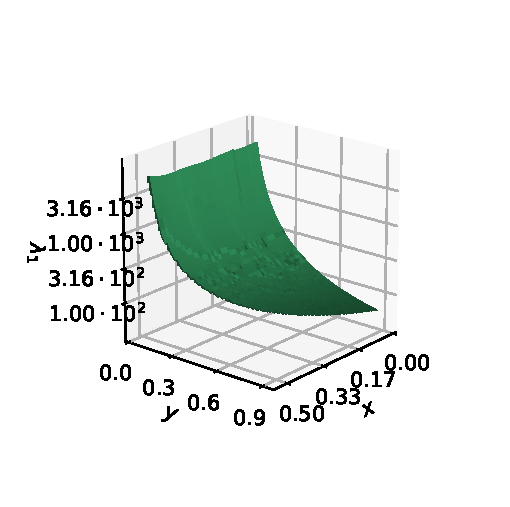
\includegraphics[width = 51.6mm]{figures/eigenvalues_3D.pdf}
                \\
                Prostorni pogled
            \end{column}
            \begin{column}{0.5\textwidth}
                \centering
                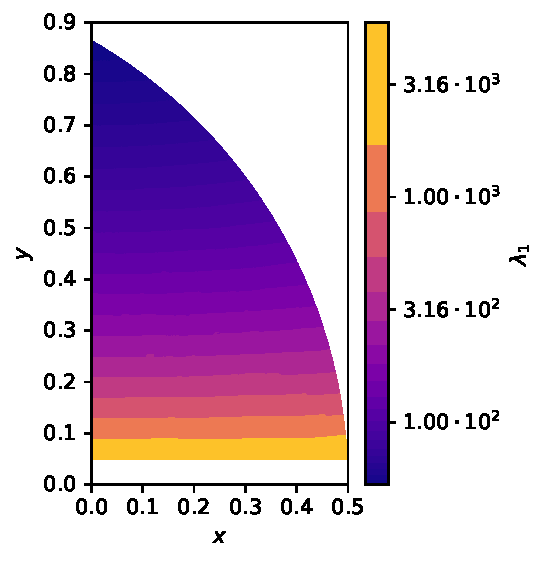
\includegraphics[width = 55.2mm]{figures/eigenvalues.pdf}
                \\
                Tlocrtni pogled
            \end{column}
        \end{columns}
    \end{frame}

    \begin{frame}{Uravnoteženje skupa podataka}
        \centering
        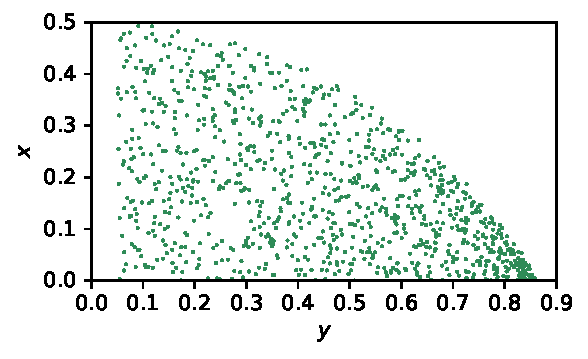
\includegraphics[width = 80mm]{figures/sample.pdf}
    \end{frame}

    \begin{frame}{Eksploratorna analiza skupa podataka}
        \only<1>{%
            \framesubtitle{Ovisnost o koordinatama karakteristične točke}

            \centering
            \begin{columns}
                \begin{column}{0.5\textwidth}
                    \centering
                    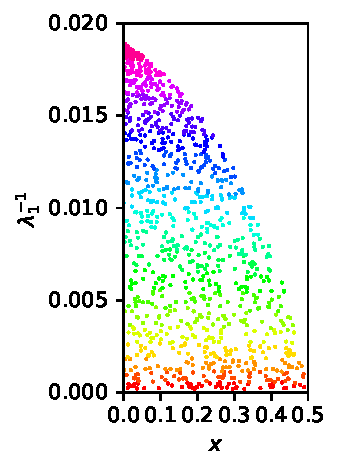
\includegraphics[width = 34.8mm]{figures/x-lambda.pdf}
                    \\
                    Apscisa
                \end{column}
                \begin{column}{0.5\textwidth}
                    \centering
                    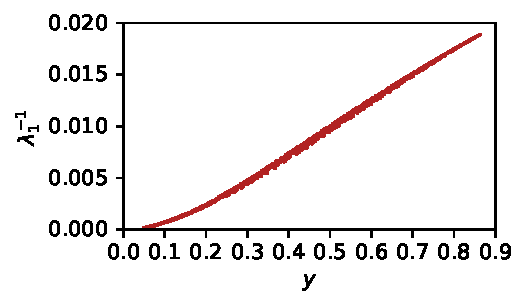
\includegraphics[width = 53.4mm]{figures/y-lambda.pdf}
                    \\
                    Ordinata
                \end{column}
            \end{columns}%
        }%
        \only<2>{%
            \framesubtitle{Ovisnost o duljinama stranica i o vanjskim kutovima}

            \centering
            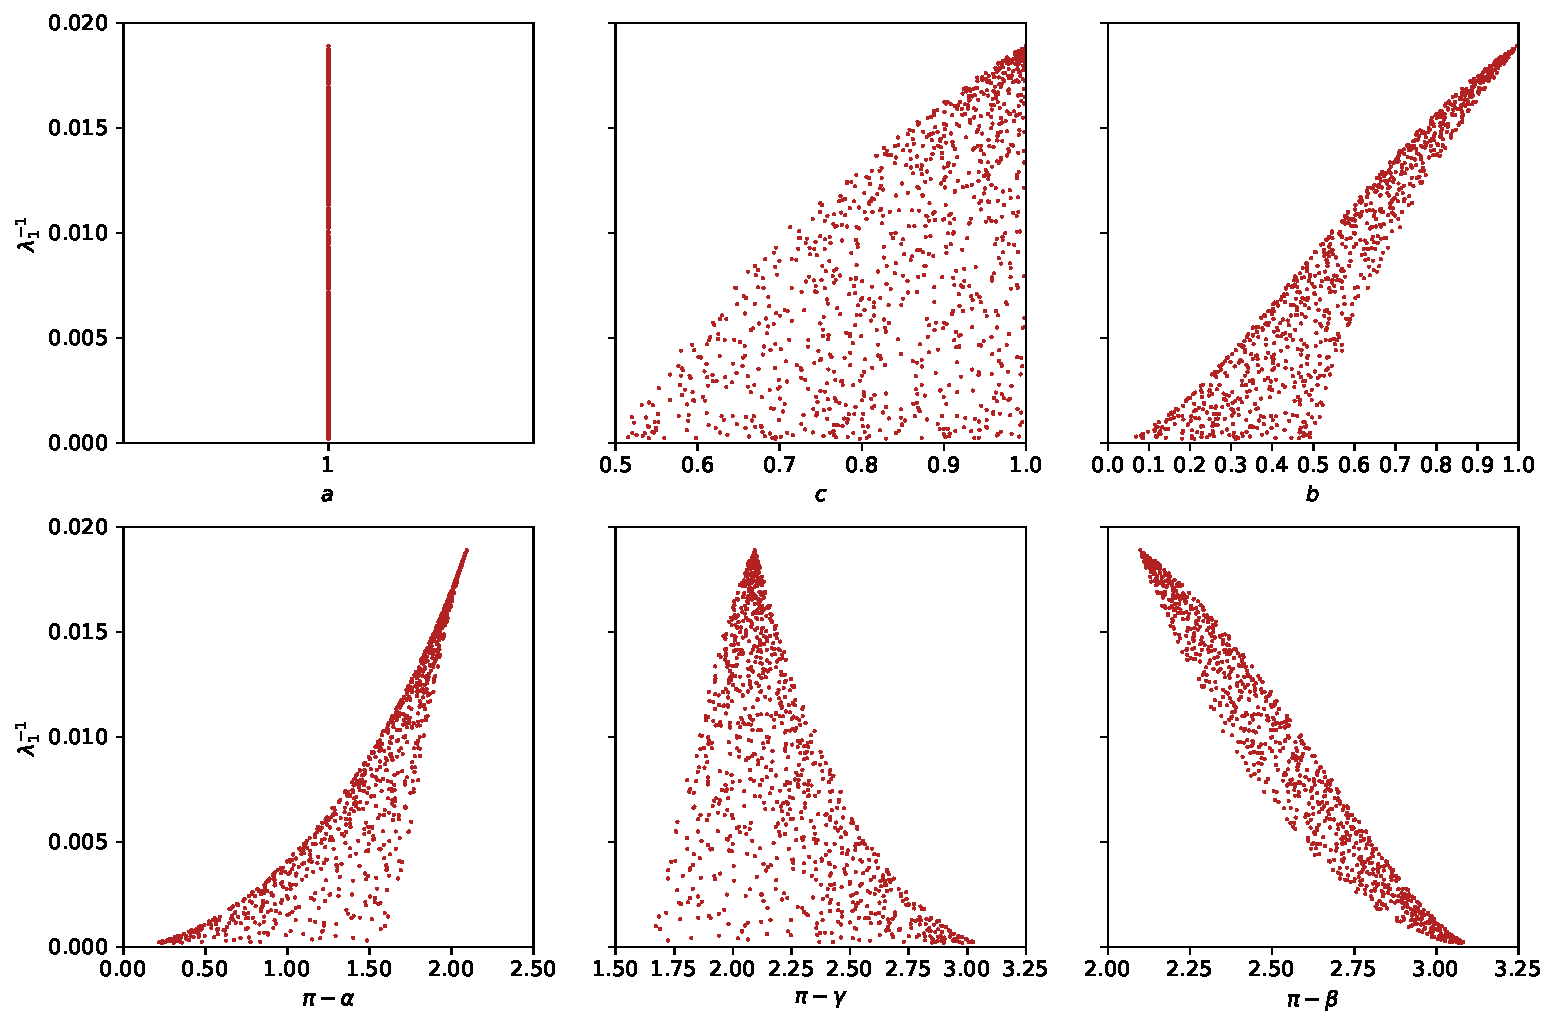
\includegraphics[width = 105.6mm]{figures/edge_angle-lambda.pdf}%
        }%
        \only<3->{%
            \framesubtitle{Ovisnost o singularnim vrijednostima duljina stranica i vanjskih kutova}

            \centering
            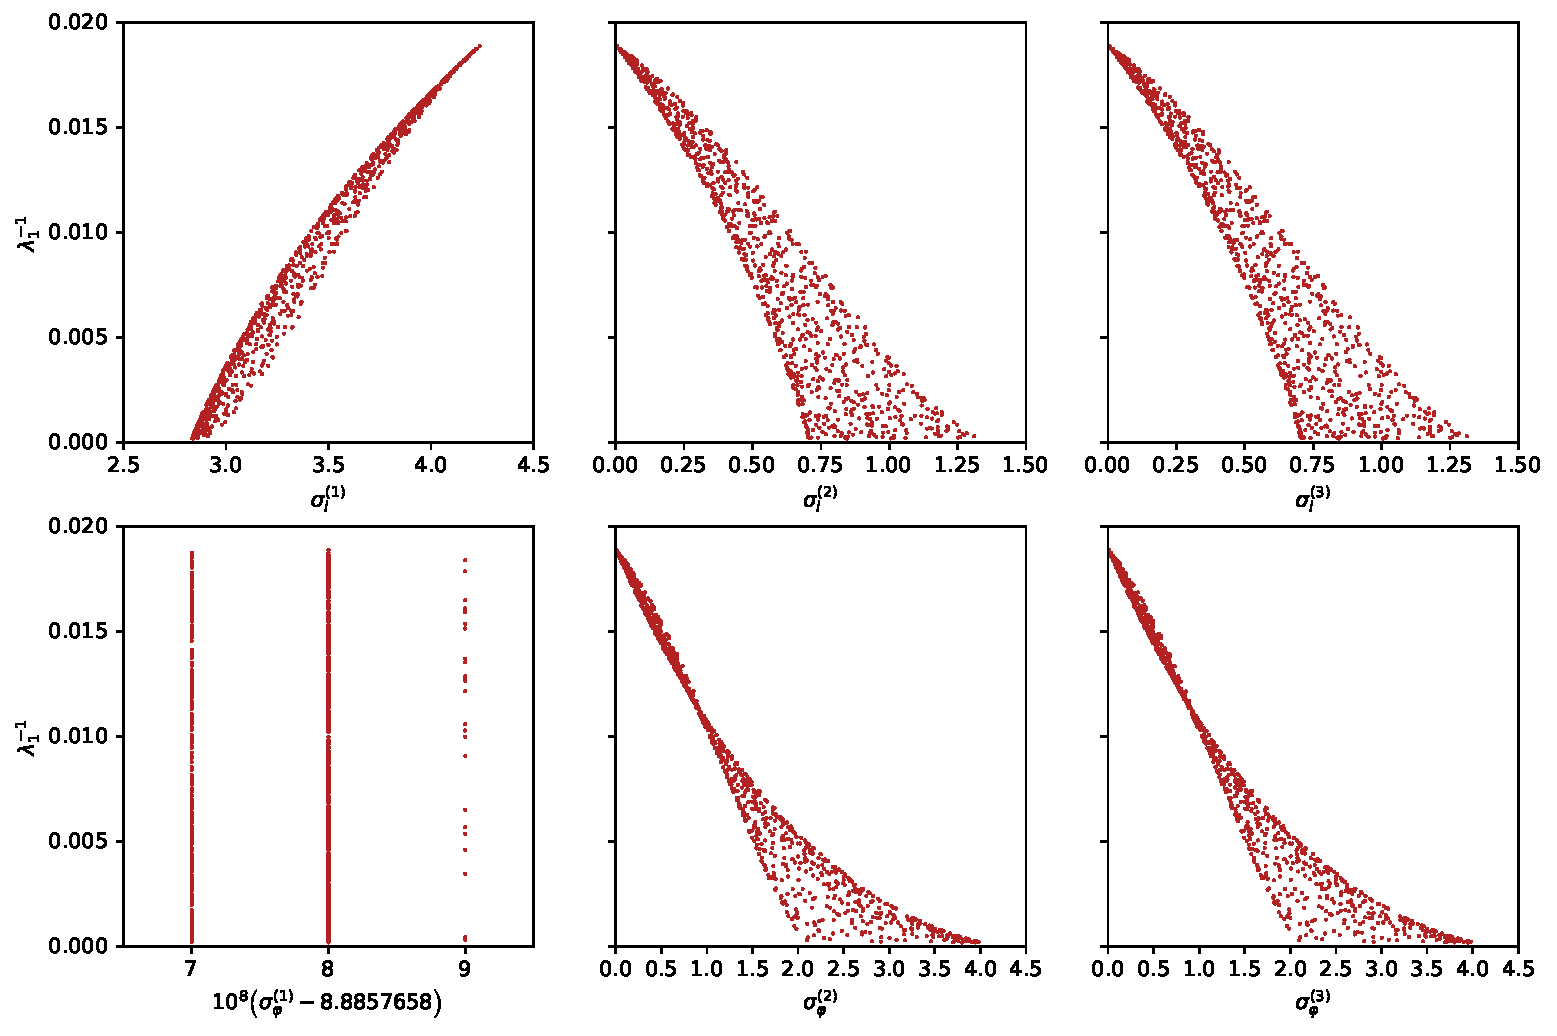
\includegraphics[width = 105.6mm]{figures/sv-lambda.pdf}%
        }%
    \end{frame}

    \section{Razvijeni modeli}

    \begin{frame}{Polinomi -- linearna regresija}

        {\small (uz konvenciju $ \numprint{0}^{\numprint{0}} \coloneqq \numprint{1} $)}
        \begin{equation*}
            P_{n} \left( x , y \right) = \sum_{k = \numprint{0}}^{n} \sum_{i = \numprint{0}}^{k} a_{i , k - i}^{\left( n \right)} x^{i} y^{k - i}
        \end{equation*}

        \par

        \begin{enumerate}
            \item $ \deftriangle{A}{B}{C} \mapsto \left( x , y \right) \in D_{{\bigtriangleup}} $
            \item $ n \in \naturals $---izbor metodom pokušaja i pogrešaka
            \item $ a_{i j}^{\left( n \right)} \in \reals $---izbor linearnom regresijom
            \item $ \lambda_{\numprint{1}}^{{- \numprint{1}}} \left( \deftriangle{A}{B}{C} \right) \approx P_{n} \left( x , y \right) $---izbor $ {{\cdot}}^{{- \numprint{1}}} $ metodom pokušaja i pogrešaka
        \end{enumerate}

        \par

        Najbolji $ n \in \left\{ \numprint{4} , \numprint{5} \right\} $

        \par
    \end{frame}

    \begin{frame}{Neuronska mreža}
        \only<1>{%
            \framesubtitle{Ulazni podatci}

            \begin{enumerate}
                \item duljine stranica u silaznom poretku---zapravo samo $ c , b $
                \item vanjski kutovi u uzlaznom poretku
                \item singularne vrijednosti duljina stranica u silaznom poretku---zapravo samo $ \sigma_{l}^{\left( \numprint{1} \right)} , \sigma_{l}^{\left( \numprint{2} \right)} $
                \item singularne vrijednosti vanjskih kutova u silaznom poretku---zapravo samo $ \sigma_{\varphi}^{\left( \numprint{2} \right)} $
            \end{enumerate}%
        }%
        \only<2>{%
            \framesubtitle{Arhitektura}

            ulaz: $ \numprint{8} $ čvorova
            \begin{enumerate}
                \item $ \numprint{16} $ čvorova---\emph{ReLU}
                \item $ \numprint{32} $ čvora---\emph{ReLU}
                \item $ \numprint{64} $ čvora---\emph{ReLU}
                \item $ \numprint{4} $ čvora---$ \text{\emph{ReLU}} \circ x \mapsto x^{{- \numprint{1}}} $
                \item $ \numprint{256} $ čvorova---\emph{ReLU}
            \end{enumerate}
            izlaz: $ \numprint{1} $ čvor%
        }%
        \only<3->{%
            \framesubtitle{Treniranje}

            \begin{itemize}
                \item \emph{adadelta}, inicijalna brzina $ \numprint{1} $
                \item \emph{MSE}
                \item $ \numprint{2000} $ epoha
            \end{itemize}%
        }%
    \end{frame}

    \begin{frame}{Konvolucijska neuronska mreža}
        Inspirirano modelom Millsa, Spannera i Tamblyna iz~\cite{bib:Mills17} za drugačiji problem diferencijalne jednadžbe

        \par

        \begin{itemize}
            \item ulazni podatci: vizualizacija dubine trokuta rezolucije $ \numprint{128} \times \numprint{128} $---u~\cite{bib:Mills17} je rezolucija $ \numprint{256} \times \numprint{256} $
            \item arhitektura:
                \begin{itemize}
                    \item $ \numprint{6} $ redukcijskih slojeva, između po $ \numprint{2} $ neredukcijska sloja---u~\cite{bib:Mills17} je $ \numprint{7} $ redukcijskih slojeva
                    \item zadnji skriveni sloj s $ \numprint{1024} $ čvora
                    \item ostali hiperparametri isti kao u~\cite{bib:Mills17}
                \end{itemize}
            \item treniranje:
                \begin{itemize}
                    \item \emph{adadelta}, inicijalna brzina $ \numprint{10}^{{- \numprint{3}}} $
                    \item \emph{MSE}
                    \item $ \numprint{50} $ epoha---u~\cite{bib:Mills17} je $ \numprint{1000} $ epoha
                \end{itemize}
        \end{itemize}

        \par
    \end{frame}

    \section{Rezultati}

    \begin{frame}{Uspješnost modela}
        \only<1>{%
            \framesubtitle{Na cijelom testnom skupu podataka}

            \centering
            \begin{columns}
                \begin{column}{0.5\textwidth}
                    \centering
                    \tiny
                    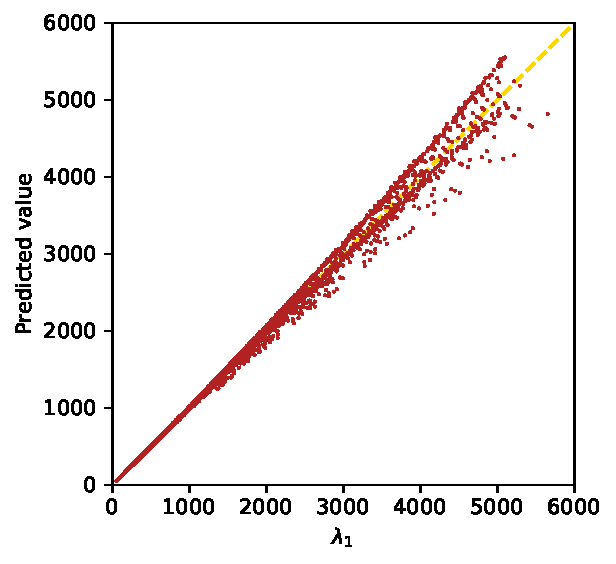
\includegraphics[width = 31.2mm]{figures/polynomial_4_prediction.pdf}
                    \\
                    $ P_{\numprint{4}} $
                \end{column}
                \begin{column}{0.5\textwidth}
                    \centering
                    \tiny
                    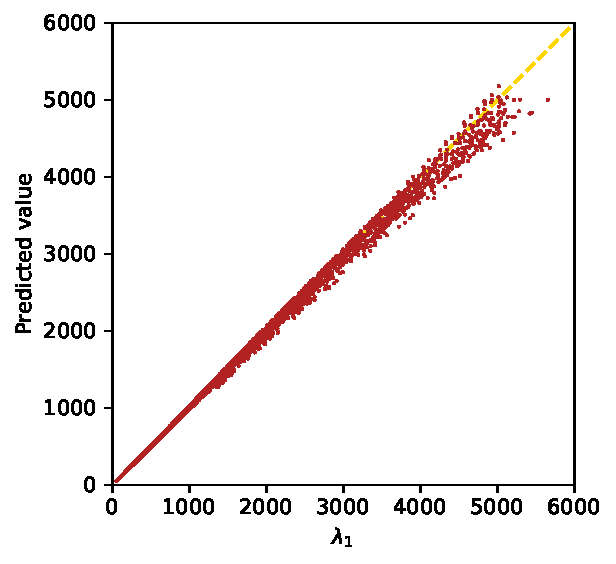
\includegraphics[width = 31.2mm]{figures/polynomial_5_prediction.pdf}
                    \\
                    $ P_{\numprint{5}} $
                \end{column}
            \end{columns}
            \begin{columns}
                \begin{column}{0.5\textwidth}
                    \centering
                    \tiny
                    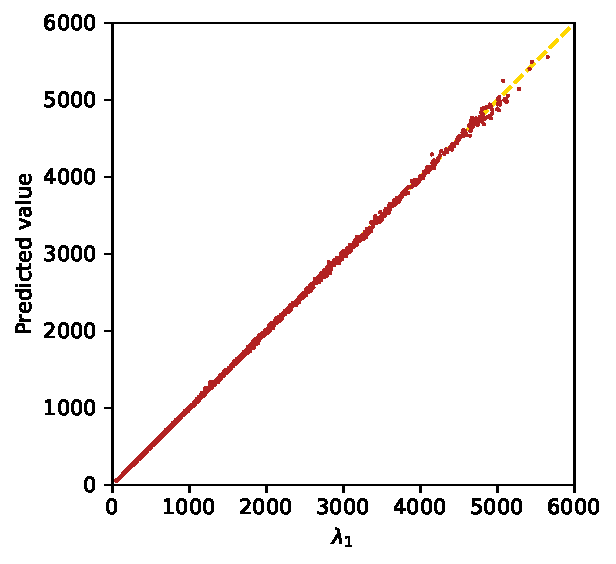
\includegraphics[width = 31.2mm]{figures/neural_network_prediction.pdf}
                    \\
                    \emph{NN}
                \end{column}
                \begin{column}{0.5\textwidth}
                    \centering
                    \tiny
                    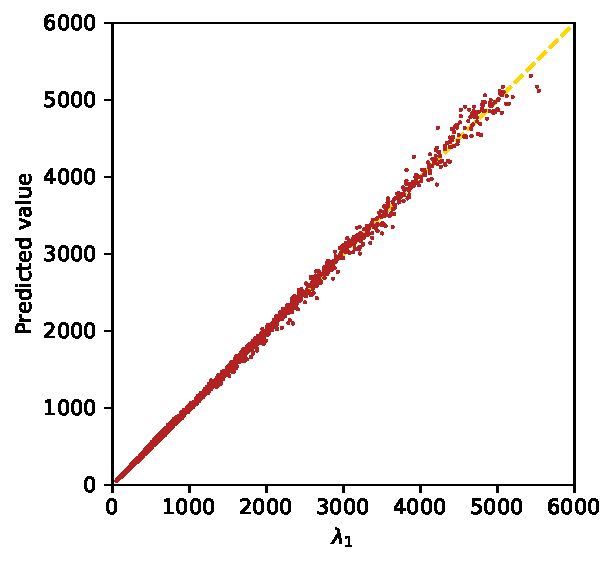
\includegraphics[width = 31.2mm]{figures/convolutional_neural_network_prediction.pdf}
                    \\
                    \emph{CNN}
                \end{column}
            \end{columns}%
        }%
        \only<2> $ vrijednosti}

            \centering
            \begin{columns}
                \begin{column}{0.5\textwidth}
                    \centering
                    \tiny
                    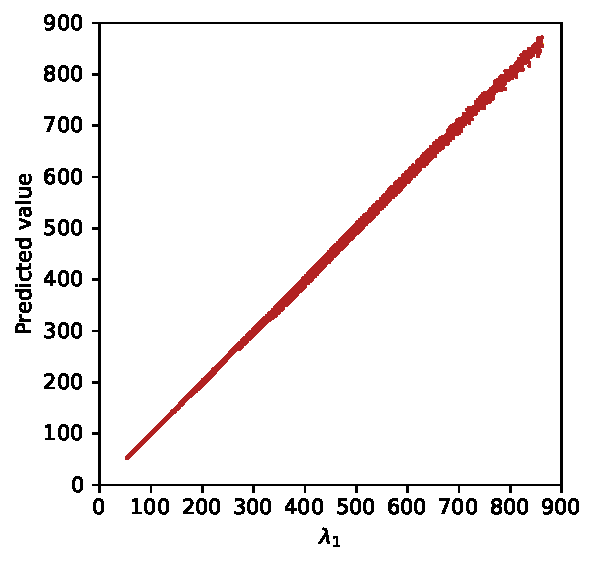
\includegraphics[width = 31.2mm]{figures/polynomial_4_prediction_90_percent.pdf}
                    \\
                    $ P_{\numprint{4}} $
                \end{column}
                \begin{column}{0.5\textwidth}
                    \centering
                    \tiny
                    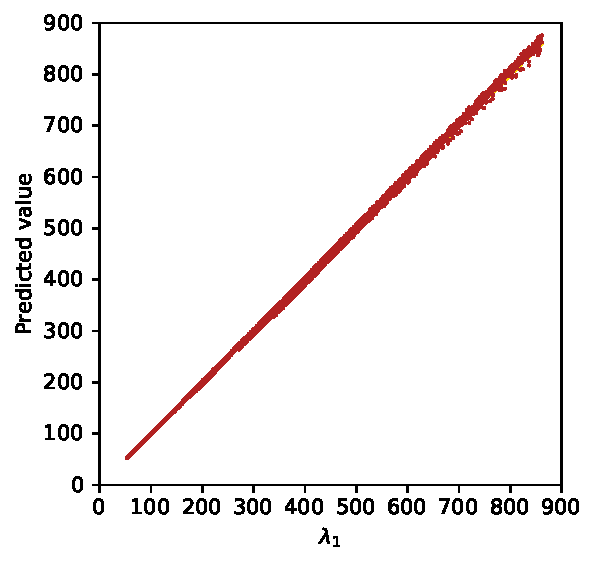
\includegraphics[width = 31.2mm]{figures/polynomial_5_prediction_90_percent.pdf}
                    \\
                    $ P_{\numprint{5}} $
                \end{column}
            \end{columns}
            \begin{columns}
                \begin{column}{0.5\textwidth}
                    \centering
                    \tiny
                    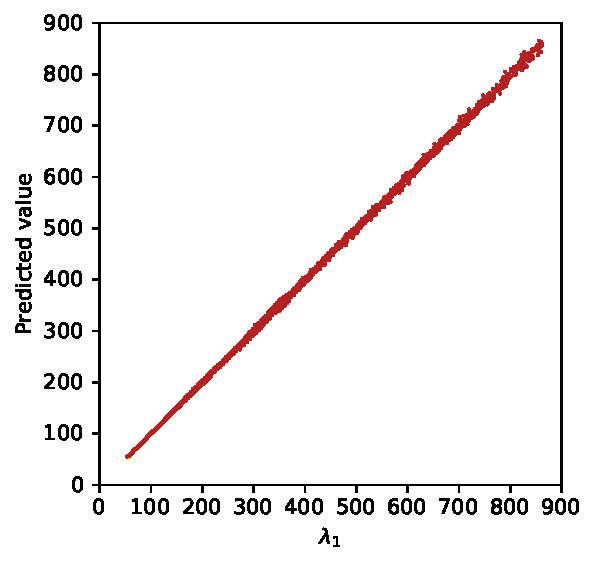
\includegraphics[width = 31.2mm]{figures/neural_network_prediction_90_percent.pdf}
                    \\
                    \emph{NN}
                \end{column}
                \begin{column}{0.5\textwidth}
                    \centering
                    \tiny
                    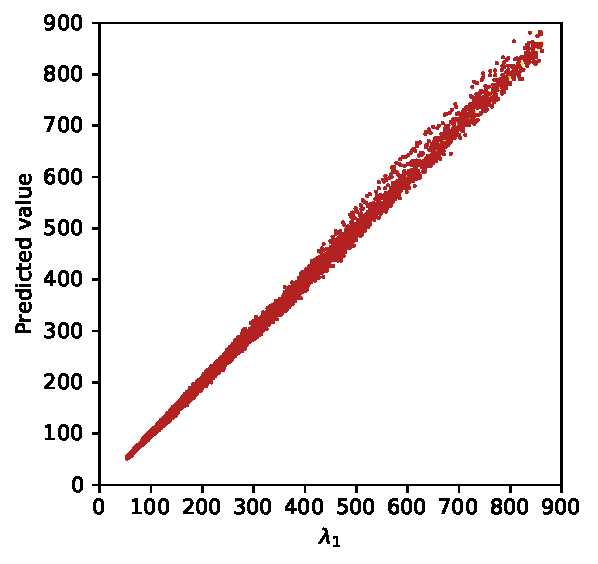
\includegraphics[width = 31.2mm]{figures/convolutional_neural_network_prediction_90_percent.pdf}
                    \\
                    \emph{CNN}
                \end{column}
            \end{columns}%
        }%
        \only<3-> $ vrijednosti}

            \centering
            \begin{columns}
                \begin{column}{0.5\textwidth}
                    \centering
                    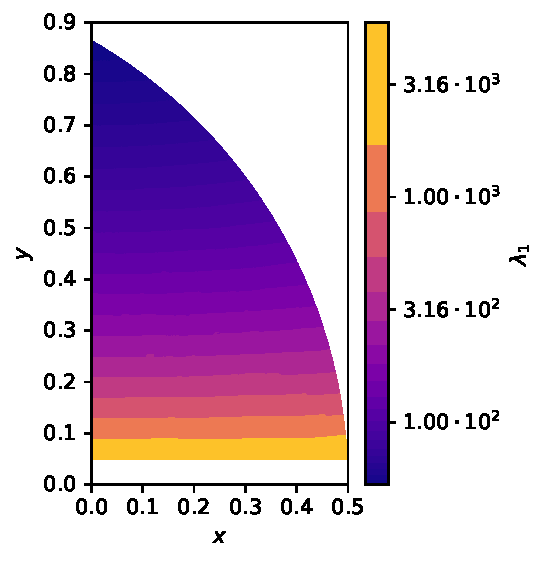
\includegraphics[width = 55.2mm]{figures/eigenvalues.pdf}
                \end{column}
                \begin{column}{0.5\textwidth}
                    Granica po ordinati za donjih
                    \begin{itemize}
                        \item[\ensuremath{\unit[\numprint{95}]{\%}}] $ y \in \intervalcc{\numprint{0.0885}}{\numprint{0.0965}} $
                        \item[\ensuremath{\unit[\numprint{90}]{\%}}] $ y \in \intervalcc{\numprint{0.1295}}{\numprint{0.1365}} $
                    \end{itemize}
                \end{column}
            \end{columns}%
        }%
    \end{frame}

    \begin{frame}{Brzina modela}
        \centering
        \begin{tabular}{| c | l | r |}
            \hline
            \multicolumn{1}{| c |}{Područje} & \multicolumn{1}{c |}{Opis} & \multicolumn{1}{c |}{Relativno vrijeme} \\
            \hline
            \multirow{1}{*}{Numerički račun} & \emph{FEM} & $ \numprint{1.000000} $ \\
            \hline
            \multirow{4}{*}{Pretprocesiranje} & Deskripcija & $ \numprint{0.000190} $ \\
             & Uređenje & $ \numprint{0.000085} $ \\
             & Karakterizacija & $ \numprint{0.000057} $ \\
             & \emph{SVD} & $ \numprint{0.005082} $ \\
            \hline
            \multirow{3}{*}{Predviđanje} & Polinom stupnja $ \numprint{4} $ & $ \numprint{0.000456} $ \\
             & Polinom stupnja $ \numprint{5} $ & $ \numprint{0.000728} $ \\
             & Neuronska mreža & $ \numprint{0.001069} $ \\
            \hline
        \end{tabular}
    \end{frame}

    \begin{frame}{Minimizacija najmanje svojstvene vrijednosti Laplaceovog operatora}
        \only<1>{%
            \begin{enumerate}
                \item varijabla $ \varphi \in \intervaloo{\numprint{0}}{\pi} $
                \item vrhovi $ A = \left( \frac{\numprint{1}}{\numprint{2}} , \numprint{0} \right) , B = \left( \cos \varphi , \frac{\sqrt{\numprint{3}}}{\numprint{2}} \sin \varphi \right) , C = \left( {- \frac{\numprint{1}}{\numprint{2}}} , \numprint{0} \right) $
                    \begin{itemize}
                        \item opseg: $ \numprint{3} $
                        \item poznata stranica: $ \linesegmentlength{C}{A} = \numprint{1} $
                    \end{itemize}
                \item minimizacija $ \lambda_{\numprint{1}} \left( \deftriangle{A}{B}{C} \right) $ po $ \varphi $
                \item cilj $ \varphi^{{*}} = \frac{\pi}{\numprint{2}} $
                    \begin{itemize}
                        \item stranice: $ \linesegmentlength{A}{B^{{*}}} = \linesegmentlength{B^{{*}}}{C} = \linesegmentlength{C}{A} = \numprint{1} $
                        \item $ \lambda_{\numprint{1}}^{{*}} \approx \numprint{52.7248} $
                    \end{itemize}
            \end{enumerate}
        }%
        \only<2>{%
            \framesubtitle{Polinom stupnja $ \numprint{4} $}

            \centering
            \begin{columns}
                \begin{column}{0.5\textwidth}
                    \centering
                    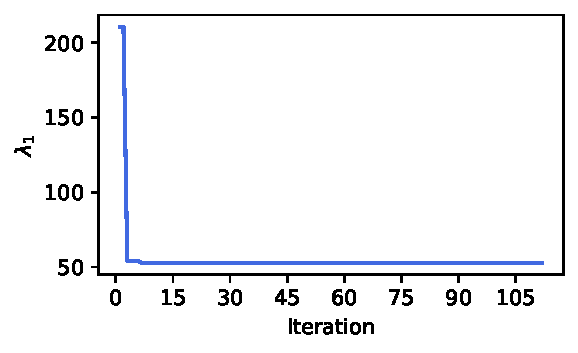
\includegraphics[width = 48mm]{figures/polynomial_4_minimisation_values.pdf}
                    \\
                    Konvergencija predviđene vrijednosti
                \end{column}
                \begin{column}{0.5\textwidth}
                    \centering
                    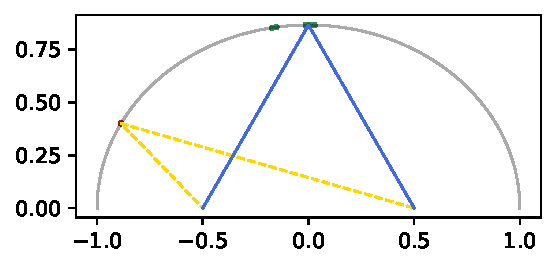
\includegraphics[width = 47mm]{figures/polynomial_4_minimisation_vertices.pdf}
                    \\
                    Konvergencija vrha
                \end{column}
            \end{columns}%
        }%
        \only<3>{%
            \framesubtitle{Polinom stupnja $ \numprint{5} $}

            \centering
            \begin{columns}
                \begin{column}{0.5\textwidth}
                    \centering
                    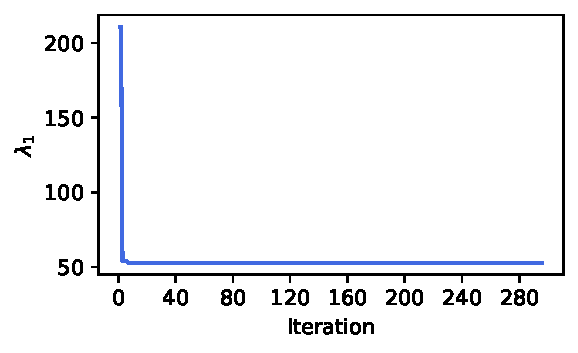
\includegraphics[width = 48mm]{figures/polynomial_5_minimisation_values.pdf}
                    \\
                    Konvergencija predviđene vrijednosti
                \end{column}
                \begin{column}{0.5\textwidth}
                    \centering
                    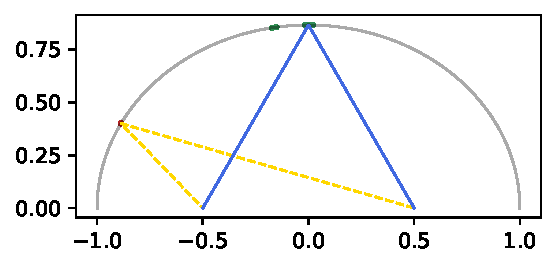
\includegraphics[width = 47mm]{figures/polynomial_5_minimisation_vertices.pdf}
                    \\
                    Konvergencija vrha
                \end{column}
            \end{columns}%
        }%
        \only<4>{%
            \framesubtitle{Neuronska mreža}

            \centering
            \begin{columns}
                \begin{column}{0.5\textwidth}
                    \centering
                    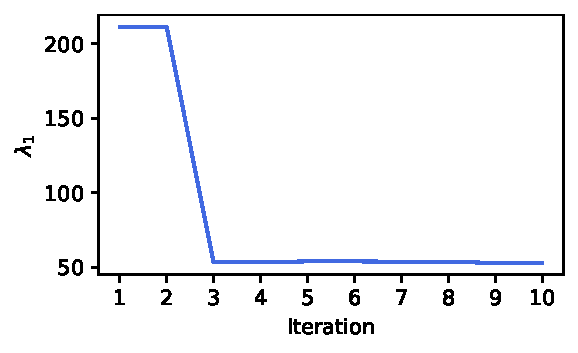
\includegraphics[width = 48mm]{figures/neural_network_minimisation_values.pdf}
                    \\
                    Konvergencija predviđene vrijednosti
                \end{column}
                \begin{column}{0.5\textwidth}
                    \centering
                    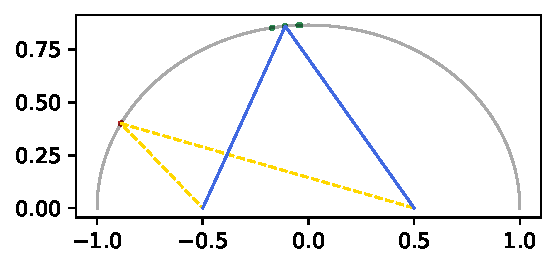
\includegraphics[width = 47mm]{figures/neural_network_minimisation_vertices.pdf}
                    \\
                    Konvergencija vrha
                \end{column}
            \end{columns}%
        }%
        \only<5->{%
            \framesubtitle{Konvolucijska neuronska mreža}

            \centering
            \begin{columns}
                \begin{column}{0.5\textwidth}
                    \centering
                    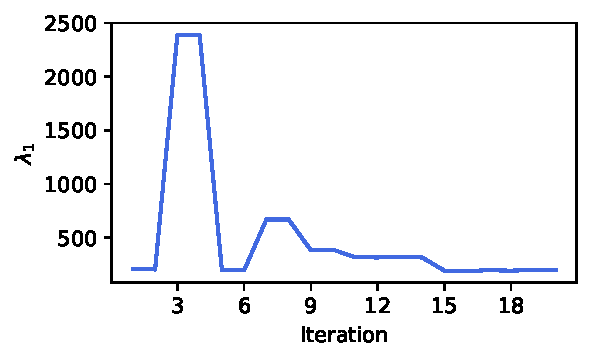
\includegraphics[width = 48mm]{figures/convolutional_neural_network_minimisation_values.pdf}
                    \\
                    Konvergencija predviđene vrijednosti
                \end{column}
                \begin{column}{0.5\textwidth}
                    \centering
                    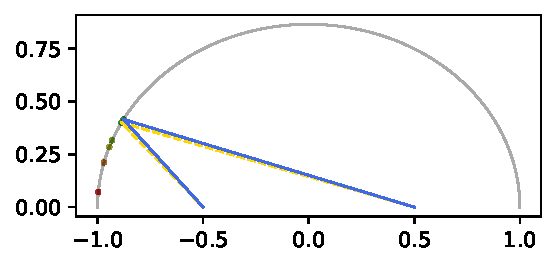
\includegraphics[width = 47mm]{figures/convolutional_neural_network_minimisation_vertices.pdf}
                    \\
                    Konvergencija vrha
                \end{column}
            \end{columns}%
        }%
    \end{frame}

    \section{Svršetak}

    \begin{frame}[allowframebreaks]
        \frametitle{Bibliografija}

        \nocite{*}
        \printbibliography[heading = none]
    \end{frame}
\end{document}
